
Aprendizado de Máquina (AM), do inglês \emph{Machine Learning}, é o estudo sistemático de algoritmos e sistemas que melhoram seu conhecimento ou desempenho com o uso da experiência \cite{flach}. Em 1959, o pioneiro em jogos de computador Arthur Samuels definiu AM como um ``campo de estudos que dá aos computadores a habilidade de aprender sem serem explicitamente programados'' \cite{simon}. De acordo com Murphy \cite{murphy} , AM pode ainda ser definido como um conjunto de métodos que conseguem detectar automaticamente padrões em dados e, em seguida, utilizar estes padrões para predizer dados não previamente vistos ou para realizar outros tipos de decisão mediante incerteza.

A essência dos métodos de AM consiste em utilizar os atributos corretos para construir os modelos certos que resolvem determinadas tarefas \cite{flach}. Os atributos são dados oriundos dos objetos relevantes no domínio do problema. Com eles, efetua-se o treinamento de um modelo para resolver um problema. Este problema é representado abstratamente por uma tarefa. Ao final do treinamento, então, o modelo é usado para endereçar a tarefa  proposta, colaborando na resolução do problema original. Estas ideias são ilustradas na Figura  \ref{fig:tasks}.

\todo{Traduzir figura.}
\begin{figure}[h!]
\centering
\caption{Uma visão geral de como ML é utilizado para endereçar uma tarefa. Adaptado de: \cite{flach}.}
\label{fig:tasks}
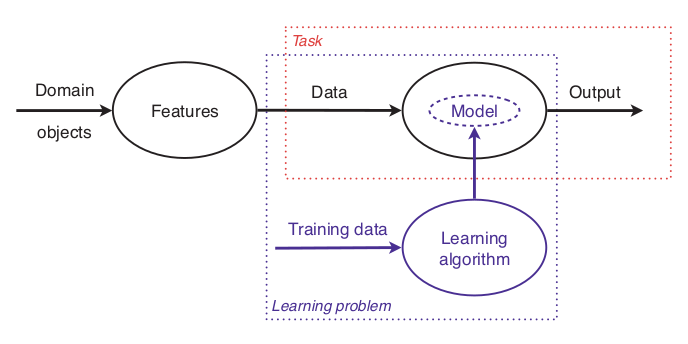
\includegraphics[width=0.7\textwidth]{imgs/tasks}
\end{figure}

A AM é comumente dividido em três paradigmas principais de aprendizado, chamados de aprendizado supervisionado, não-supervisionado e semi-supervisionado. No caso dos algoritmos de aprendizado supervisionado, o objetivo é aprender um mapeamento de entradas para saídas, dado um conjunto rotulado de pares de entradas e saídas. No aprendizado não supervisionado, o algoritmo é apresentado somente aos dados de entrada e o seu propósito é encontrar padrões significativos nos mesmos. O aprendizado semi-supervisionado, por sua vez, normalmente combina uma pequena quantidade de dados rotulados com uma grande quantidade de dados não rotulados para criar um classificador próprio a ser aplicado aos dados não rotulados. Em alguns casos, a abordagem de aprendizado semi-supervisionado pode ser de grande valor prático \cite{khan}.

No caso do paradigma de aprendizado supervisionado, em particular, destacam-se as tarefas de classificação e de regressão. Em uma tarefa de classificação, um algoritmo é selecionado para especificar quais das $k$ categorias possíveis uma entrada pertence. Para resolver essa tarefa, o algoritmo de aprendizado normalmente produz uma função $f : \mathbbm{R}^n \rightarrow \{1, \ldots, k\}$. Quando $y = f(x)$, isto significa que o modelo mapeia uma entrada descrita pelo vetor $x \in \mathbbm{R}^n$ para uma categoria identificado por um valor numérico $y \in \{1, \ldots, k\} $ \cite{goodfellow}. [Alguns exemplos de tarefa de classificação são a detecção de faces em imagens, a determinação do gênero do indíviduo nessas imagens, a verificação da espécie de uma planta, entre outros.] \todo{Rever exemplos}

Quanto à tarefa de regressão, é solicitado a um algoritmo de AM a predição de um valor numérico a partir de uma entrada. Desta forma, o algoritmo de aprendizado é proposto a inferir uma função $f : \mathbbm{R}^n \rightarrow \mathbbm{R}$ \cite{goodfellow}. [Algumas tarefas de regressão podem ser, por exemplo, a determinação do valor de uma corrida de táxi, a identificação da idade de um indivíduo em uma imagem \todo{Citar trabalho da Nicoli}, prever o preço de uma casa baseado nos dados de casas vendidas anteriormente, etc.] \todo{Citar Marsland?}

Dentre os diversos modelos de AM existentes, Flach considera a categorização dos mesmos segundo os tipos geométricos, probabilísticos e lógicos \cite{flach}. Modelos geométricos são construídos diretamente. Um modelo geométrico é construído diretamente em função do espaço da solução, utilizando-se de conceitos como linhas, planos, hiperplanos e distâncias. Nesta categoria encontram-se a regressão linear, as redes neurais artificiais e as máquinas de vetores de suporte, por exemplo. Nos modelos do tipo probabilísticos, como o classificador Bayesiano, por exemplo, a questão principal é modelar a relação entre os dados de entrada e de saída assumindo que existe algum processo aleatório implícito que produz os valores para essas variáveis, de acordo com uma distribuição de probabilidade bem definida, porém desconhecida. Um modelo lógico, por sua vez, é o mais naturalmente algorítmico, considerando a capacidade de ser facilmente transformado em regras que podem ser entendidas por seres humanos. Dentre os modelos lógicos estão, por exemplo, as árvores de decisão e as florestas aleatórias.

\todo[inline]{Construir transição sutil para próxima seção. Sugestão: citar vários exemplos de problemas resolvidos com AM. Na próxima seção serão descritas e apresentadas as RNAs, um dos modelos de AM para aprendizado supervisionado com papel protagonista nas soluções apresentadas.}

%%Dentre os modelos geométricos, as redes neurais artificiais têm demonstrado grande desempenho em diversas áreas. Aplicações de \emph{Deep Learning} para detecção de padrões em imagens e reconhecimento de voz, por exemplo, utilizam-se desses modelos para a obtenção de resultados relevantes. Tomando isto e levando em consideração o contexto deste trabalho, as próximas seções apresentadas abordam significativamente estes conceitos.

%%%%%
